% !TeX spellcheck = sl_SI
\documentclass[a4paper,notumble]{leaflet} % 


\usepackage[T1]{fontenc}
\usepackage[utf8]{inputenc}
\usepackage[slovene]{babel}
\usepackage{amsmath}
\usepackage[scaled=0.9]{helvet}
\usepackage[bookmarks, colorlinks=true, linkcolor=black, anchorcolor=black, citecolor=black, filecolor=black, menucolor=black, runcolor=black, urlcolor=black, pdfencoding=unicode]{hyperref}
\usepackage{fontawesome}

\hyphenation{pred-no-vo-let-nem}

% \setmargins{1cm}{1cm}{0.5cm}{0.5cm}

% \CutLine*{1}% Dotted line without scissors

\begin{document}
  \begin{center}
    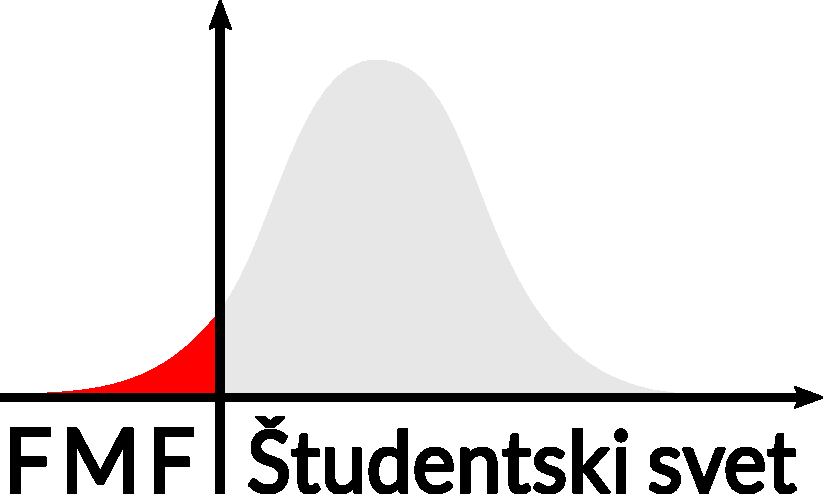
\includegraphics[width=0.6\linewidth]{ssfmf_logo_col.pdf}
    
    \vfill
    
    \textbf{\Huge Študentski svet} \\[0.2cm]
    \textbf{Fakultete za matematiko in fiziko} \\ [1cm]
    
    predstavlja \\[1cm]
    
    \textbf{\LARGE Vodič v \\[0.2ex] študijsko in obštudijsko \\[1ex]  življenje na FMF}
    
    \vfill
    \vfill
    \vfill
    
    
  \end{center}
  \newpage 
  \section{Kaj je študentski svet?}
  Študentski svet (ŠS) je organ študentov v okviru fakultete. Je edini organ, ki uradno predstavlja študente znotraj fakultete in na višjem nivoju še znotraj Univerze. Smo vez med študenti in fakulteto. \textbf{Vsak študent se lahko na ŠS obrne s kakršno koli težavo ali vprašanjem študijske ali socialne narave. Obravnavali ga bomo resno in svetovali po najboljših močeh ter ga po potrebi usmerili na drug, bolj primeren organ ali osebo.}
  
  ŠS sestavljamo študentje, in sicer od 9 do 13 izvoljenih predstavnikov.
  Mesečno se svet dobiva na rednih sejah, kjer obravnava tekočo tematiko. Sodelovanje v ŠS je prostovoljno (ni plačano).
  
  \vspace{-2ex}
  \section{Dejavnosti ŠS}
  Študenti imamo predstavnike skoraj v vseh organih fakultete:
  Senatu, Znanstveno-pedagoških svetih, Akademskem zboru, 
  Upravnem odboru, Disciplinski komisiji, Komisiji za študijske zadeve, Komisiji za kakovost in Komisiji za etična vprašanja.
  
  Ena izmed pomembnejših nalog sveta je, da podajamo študentska mnenja o zaposlenih na fakulteti
  ob izvolitvi v naziv. Samo s pozitivnim mnenjem ŠS
  lahko zaposleni naprej uči na fakulteti. Mnenja pišemo na podlagi 
  anket, ki jih za vsak predmet izpolnite v sistemu VIS. 
  
  \vspace{-2ex}
  \section{Življenje na FMF}
  Na FMF imamo nekaj dejavnosti, ki jih organizira ŠS FMF
  ali pa zainteresirani študenti sami. Ponavadi se dejavnosti oglašujejo 
  na oglasnih deskah pri dvigalih, nekaj pa jih je že stalnih:
  \begin{description}
    \item[$\boldsymbol \pi$-dan] je 14.\ marec, ko se na FMF dogaja tekmovanje
    v recitiranju decimalk števila $\pi$.
    \item[FMF hoodie-ji] se naročijo vsako leto okoli februarja in z njimi lahko pokažeš svojo pripadnost.
    \item[Novoletna stojnica] je organizirana v prednovoletnem času in ponuja sveže pečene
    toaste in kuhane napitke. Okrašuje se tudi novoletna jelka.
    \item[Družabni večeri] so organizirani približno enkrat na mesec v Ma$\varphi$ji, 
    kjer imamo študenti čas za klepet in sprostitev ob igranju družabnih iger. 
    \item[Čajni kotiček] se nahaja v tretjem nadstropju stavbe za matematiko, kjer je zraven avtomata za vročo vodo tudi zbirka čajev in dobrot.
    \item[Knjižni klub] se sestaja nekajkrat letno in se pogovarja na vsakem 
    srečanju o vnaprej dogovorjeni knjigi. Glej oglasne deske pri dvigalih za več informacij.
  \end{description}
  \vspace{-1ex}
  \section{Učenje}
  Veliko študentov ima težave s snovjo
  v prvih letnikih. Pomoč lahko najdete na več mestih:
  \begin{description}
    \item[Sošolci:] ravno vaši sošolci najbolje vedo,
    kaj točno je profesor ali asistent napisal na vajah
    ali predavanjih in skupno odkrivanje bistva je del učnega procesa.
    \item[Tutorstvo:] tutorji so študenti višjih letnikov, ki so pripravljeni svoje znanje in izkušnje organizirano in prostovoljno deliti z mlajšimi. Vsak tutor je eno uro na teden na voljo za vsa vprašanja (glede snovi ali drugih stvari) in velikokrat je lažje razumeti študenta, ki je pred kratkim imel enako izkušnjo, kot profesorja ali asistenta. Na fiziki je tutorstvo vezano na predmete.
    Oglej si predmet ``Tutorstvo'' na spletni učilnici za več informacij.
    \item[Zapiski:] če nimaš zapiskov, lahko pogledaš na \url{zapiski.fmf.si}, kjer najdeš skenirane zapiske prejšnjih generacij. Lahko tudi dodaš svoje!
    \item[Forum:] namesto v živo lahko vprašaš svoje vprašanje tudi na \url{forum.fmf.si}. Forum aktivno gledajo tudi tutorji in se ga pogosto uporablja za pomoč pri reševanju nalog.
  \end{description}
  Za učenje je v četrtem nadstropju stavbe za matematiko nekaj ``kletk'' (steklenih prostorov
  z mizami in tablami, namenjenimi učenju). Poleg tega je nekaj prostora tudi v tretjem in drugem nadstropju. Skupna soba v četrtem nadstropju je namenjena zaposlenim. Na fiziki je v pritličju študentska soba, nekaj prostora je tudi v višjih nadstropjih.
  
  \vspace*{-2ex}    
  \section{Mafijski piknik}
  Mafijski piknik je največji družabni dogodek na FMF, ki ga ŠS FMF tradicionalno organizira sredi maja v Mostecu. 
  Je piknik s približno 600 udeleženci, med katerimi smo študenti, profesorji in asistenti na FMF. Z vstopnico dobiš
  majico piknika in ``neomejeno'' pijačo ter hrano.
  Poleg tega so organizirane športne aktivnosti, med drugim tudi tradicionalno vlečenje 
  vrvi med matematiki in fiziki. Glasba, ples, zabava in pogovarjanje pa trajajo krepko v naslednji dan.
  Če želiš sodelovati pri pripravi letošnjega piknika, spremljaj našo Facebook stran, kjer bomo objavili natečaj za dizajn letošnjega motiva majice in poziv za prostovoljce.
  
  \vspace{-2ex}
  \section{Tehnika in komunikacija}
  \vspace{-1ex}
  Za komunikacijo s fakulteto, profesorji in asistenti uporabljajte uradni email naslov oblike
  \url{ime.priimek@student.fmf.uni-lj.si}, ki ste ga dobili ob vpisu. Ta naslov morate tudi redno pregledovati. Pri FMF pošti si lahko nastavite, da se prejeta sporočila posredujejo na nek drug naslov. Prav tako lahko pri nekaterih ponudnikih (npr.\ Gmail) nastavite, da lahko pošiljate z drugih naslovov.
  Priporočamo, da se na FMF strani naročite na obvestila, da boste obveščeni o vpisnih rokih in spremembah urnikov.
  
  Vsak študent ima na voljo tudi točke za tiskanje. Tiskalniki so v sobah 3.08 in 3.09 na matematiki in v računalnici na fizki. Za tiskanje se morate na tiskalnik vpisati s svojim uporabniškim računom, ki ga lahko povežete tudi z urbano, da vam ni treba vsakič vpisovati uporabniškega imena in gesla.  Za registracijo urbane jo samo približajte čitalcu kartic in sledite navodilom, vsakič naslednjič pa se preprosto vpišete samo z urbano.
  
  Za več informacij glede tehnologije (VIS, Eduroam) glejte strani Računalniškega centra FMF, spletno učilnico Računalniškega praktikuma (RP) ali pa za pomoč vprašajte starejše študente ali asistenta pri RP.
  
  V tutorski kletki v tretjem nadstropju stavbe za matematiko imate tudi pisarniške pripomočke za skupno uporabo, med drugim tudi napravo in potrebščine za vezanje nalog.
  
%  \vfill \hfill
%  \textit{Želimo vam veliko uspeha pri študiju.}
  
  \newpage
  \newpage
  {\Large
    
    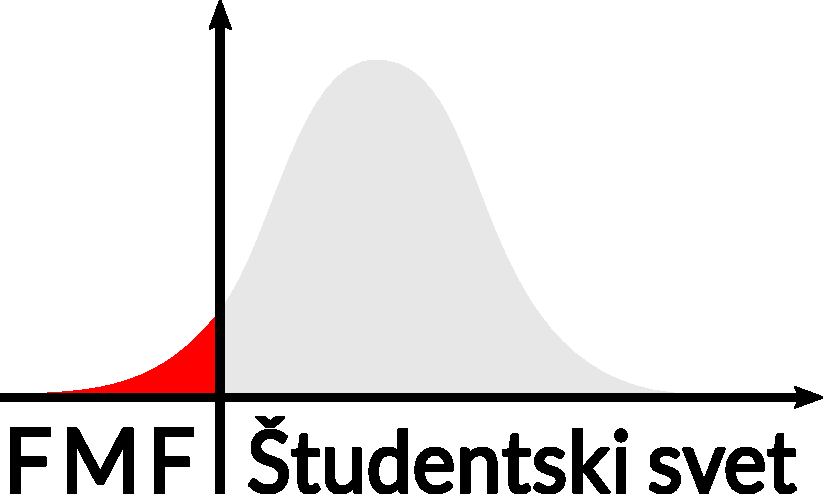
\includegraphics[width=0.6\linewidth]{ssfmf_logo_col.pdf} \\[1cm]
    
    Študentski svet \\
    Fakulteta za matematiko in fiziko \\
    Jadranska ulica 19 \\
    1000 Ljubljana \\[1cm]
    
    \begin{tabular}{cl}
      \faBuilding{} & stavba matematike, soba 2.06 \\[0.3cm]
      \faGlobe{} & \url{svet.fmf.si} \\[0.3cm]
      \faEnvelopeSquare{} & \url{studentski.svet@fmf.uni-lj.si} \\[0.3cm]
      \faFacebookSquare{} & \url{fb.com/Studentski.svet.FMF}
    \end{tabular}
    
  }
  
  \vfill
  verzija: 1.~10.~2019
\end{document}